\documentclass[a4paper]{article}
\usepackage{sst2022,amssymb,amsmath,epsfig}
\usepackage[hidelinks]{hyperref}
\setcounter{page}{1}
\sloppy     % better line breaks
\ninept
%SM below a registered trademark definition
\def\reg{{\rm\ooalign{\hfil
     \raise.07ex\hbox{\scriptsize R}\hfil\crcr\mathhexbox20D}}}


%% \newcommand{\reg}{\textsuperscript{\textcircled{\textsc r}}}
\title{Abstract Template for SST 2022 -- Canberra, ACT, Australia}

%%%%%%%%%%%%%%%%%%%%%%%%%%%%%%%%%%%%%%%%%%%%%%%%%%%%%
%% If multiple authors, uncomment and edit the lines shown below.       %%
%% Note that each line must be emphasized {\em } by itself.             %%
%% (by Stephen Martucci, author of spconf.sty).                         %%
%%%%%%%%%%%%%%%%%%%%%%%%%%%%%%%%%%%%%%%%%%%%%%%%%%%%%
%\makeatletter
%\def\name#1{\gdef\@name{#1\\}}
%\makeatother
%\name{{\em Firstname1 Lastname1, Firstname2 Lastname2, Firstname3 Lastname3,}\\
%      {\em Firstname4 Lastname4, Firstname5 Lastname5, Firstname6 Lastname6,
%      Firstname7 Lastname7}}
%%%%%%%%%%%%%%% End of required multiple authors changes %%%%%%%%%%%%%%%%%

\makeatletter
\def\name#1{\gdef\@name{#1\\}}
\makeatother \name{{\em XXX}}

\address{XXX\\
{\small \tt XXX}}

%
\begin{document}
\maketitle
%
\noindent{\bf Index Terms}: speech synthesis, unit selection, join costs

%
\section{Introduction}

This template can be found on the conference website. To ensure compliance with the layout specifications, please use either the MS-Word\reg\ or \LaTeX\ format template when preparing your
submission. 
Both templates are available through the conference website:\\\href{https://sst2022.com/}{https://sst2022.com/}.\\Please contact the conference organising committee at sst2022conf@gmail.com with any questions.

\subsection{Layout requirements}

\begin{itemize}
\item Abstracts submitted must be formatted for A4 paper.
\item A maximum of one page is allowed for the abstract.
\item Text in the main body of the abstract should be 9 point Times or Times Roman font.
\item A 5-section structure (Introduction, Methodology, Results, Discussion, References) is recommended.
\item The submitted file must be in PDF format, with no password protection.
\end{itemize}

\subsection{Tables and figures}

An example of a table is shown in Table \ref{table1}, and an example of a figure is shown in Figure \ref{spprod} 

\begin{table} [thb]
\caption{\label{table1} {\it Figure and table caption text should be italicized.}}
\vspace{2mm}
\centerline{
\begin{tabular}{|c|c|}
\hline
ratio & decibels \\
\hline  \hline
1/1 & 0 \\
2/1 & $\approx 6$ \\
3.16 & 10 \\
10/1 & 20 \\
1/10 & -20 \\
100/1 & 40 \\
1000/1 & 60 \\
\hline
\end{tabular}}
\end{table}

\begin{figure}[thb]
\centerline{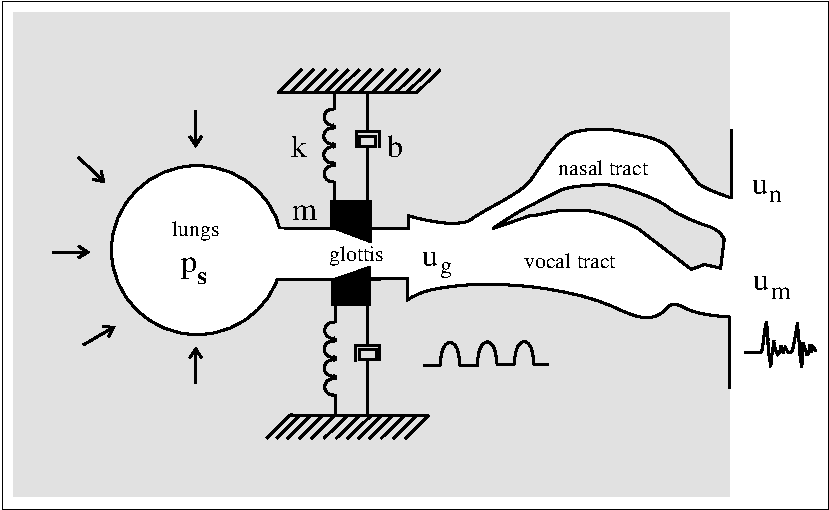
\epsfig{figure=figure,width=80mm}}
\caption{{\it Schematic diagram of speech production.}}
\label{spprod}
\end{figure}

\subsection{Equations}

Equations should be placed on separate lines and numbered. Examples
of equations are given below.
Specifically,

\begin{equation}
x(t) = s(f_\omega(t)),
\label{eq1}
\end{equation}
where \(f_\omega(t)\) is a special warping function
\begin{equation}
f_\omega(t)=\frac{1}{2\pi j}\oint_C \frac{\nu^{-1k}d\nu}
{(1-\beta\nu^{-1})(\nu^{-1}-\beta)}.
\label{eq2}
\end{equation}

\subsection{References}

References should be formatted according to the IEEE standards.
References should be numbered in order of appearance,
for example \cite{ES2}, \cite{ES3},  \cite{ES4}, and \cite{ES5}.

\section{Anonymity}

The review process for SST2022 will be anonymous. As such, the names of the authors and affiliations should not be mentioned in either the title or the text of the paper during the initial round of submissions. Further, any references to the authors' previous research should be made as anonymous as possible.  For instance, instead of ``In our previous study \cite{ES2}, we show that\ldots'' use ``As shown previously in \cite{ES2}\ldots''
Work that the authors have submitted for publication but has not yet been published should be referenced as ``anonymous,'' as in \cite{ES5}.
Also ensure that no author details appear in the Document Properties of the PDF file.

In the revised submission round, authors' details should be added.  if an abstract has multiple authors, all authors' names should be followed by a superscript numeral, while the respective affiliations should be preceded by the corresponding superscript.

%
\eightpt
\bibliographystyle{IEEEtran}
\begin{thebibliography}{10}
\bibitem[1]{ES2} Soquet, A., Saerens, M. and Jospa, P., ``Acoustic-articulatory
inversion'', in T. Kohonen [Ed], Artificial Neural Networks, 371-376,
Elsevier, 1991.
\bibitem[2]{ES3} Stone, H.S., ``On the uniqueness of the convolution theorem
for the Fourier transform'', NEC Labs. Amer. Princeton, NJ.
Online: http://citeseer.ist.psu.edu/176038.html, accessed on 19 Mar 2008.
\bibitem[3]{ES4} Fant, G., Acoustic Theory of Speech Production, Mouton, 1960.
\bibitem[4]{ES5} Anonymous, ``Some study that has not yet been published'', submitted.
\end{thebibliography}
\end{document}
